\documentclass[tikz,border=3.14mm]{standalone}
\begin{document}
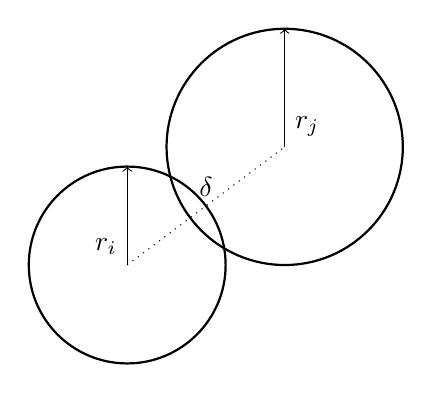
\begin{tikzpicture}

% Define coordinates
\coordinate (ri) at (0, 0); % Center of first circle
\coordinate (rj) at (2, 1.5); % Center of second circle

% Draw circles
\draw[thick] (ri) circle(1.25cm) node[above left] {$r_i$};
\draw[thick] (rj) circle(1.5cm) node[above right] {$r_j$};

% Draw connecting line and label
\draw[dotted] (ri) -- (rj) node[midway, above] {$\delta$};

% Draw arrows for radius
\draw[->] (ri) -- ++(0,1.25);
\draw[->] (rj) -- ++(0,1.5);

\end{tikzpicture}
\end{document}
